\section{Motivation}
Modern machine learning algorithms have reached a degree of potential that lets the resulting models model almost any data set.
But even though there are statistical measures to guarantee that the model is learning correctly without over-fitting on the training data, the model with the highest accuracy is not always the most usable model or even semantically correct.
The following three examples aim to showcase this:

\par \noindent (1)
Caruana~\etal\cite{Caruana:2015:IMH:2783258.2788613} built a Generalized Additive Model with pairwise interaction ($GA^2M$) to predict mortality risk for hospitalized patients with pneumonia, a potentially life-threatening lung infection. This area of machine learning is called predictive modeling and uses machine learning to predict a certain outcome, in this case mortality risk, based on values of several input features, in this case laboratory measurements, comorbidities, or patient demographics, and is trained from and applied to many instances. It is not feasible to individually check each prediction of the model manually. However, the machine learning algorithm $GA^2M$ used for this study is an intelligible model, that sacrifices parts of its predictive quality in favor of being understandable by humans. This enabled the authors to inspect how features contributed to the predicted outcome. One of their findings was that the model associated having asthma, a chronic lung disease, with a lower mortality rate for pneumonia patients. However, this combination of diseases is known to have a significantly \emph{increased} mortality rate. The authors double checked their data and found that this phenomenon actually occurred in their dataset and thus appeared as correct prediction in their model. After further investigation it became clear that this bias in the dataset stemmed from patients, with those conditions, being treated with intensive care thus lowering their mortality risk below the average. Outside of a hospital the risk of those patients would have been significantly higher. The model, however, only learnt about hospitalized patients which led to it being confident in this false association.

\begin{figure}
\centering
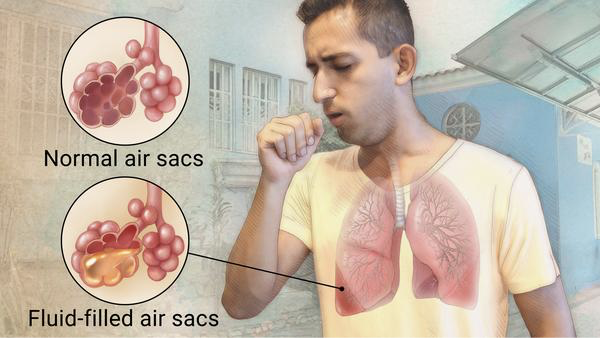
\includegraphics[height=6em,valign=t]{tex/introduction/pneumonia.png}
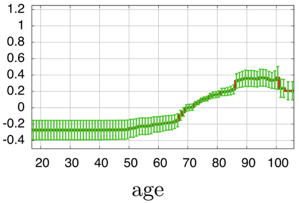
\includegraphics[height=8em,valign=t]{tex/introduction/age.png}
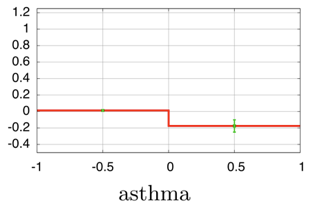
\includegraphics[height=8em,valign=t]{tex/introduction/asthma.png}
\caption[Influence functions of Pneumonia model.]{
Pneumonia is an infectious disease of the lungs that inflames air sacs and likely fills them with fluid, making it hard to breathe and potentially life-threatening (left\footnotemark).
The influence functions of the features ``age" (middle) and ``asthma" (right) of the model created by Caruana~\etal\cite{Caruana:2015:IMH:2783258.2788613}.
}
\label{figs:pneumonia}
\end{figure}
\footnotetext{Image source: Google}

\par \noindent (2)
Layzell and Bird \cite{Bird:2002:ERI:1251972.1252349} used machine learning to automatically design an oscillator, an electronic circuit that produces a periodic oscillating signal, using a physical programmable circuit rather than a simulated circuit. After the model completed the task, the scientists looked at the resulting electronic circuit and were surprised to find that instead of the conventional design, using a feedback loop of an amplifier and a filter, the model designed a makeshift radio that responded to the desired frequency and amplified radio signals emitted by nearby computers instead. The output signal of this electronic circuit had the correct frequency and amplitude according to the specification but did not create a valid result due to a latent bias in the available data.

\begin{figure}
\centering
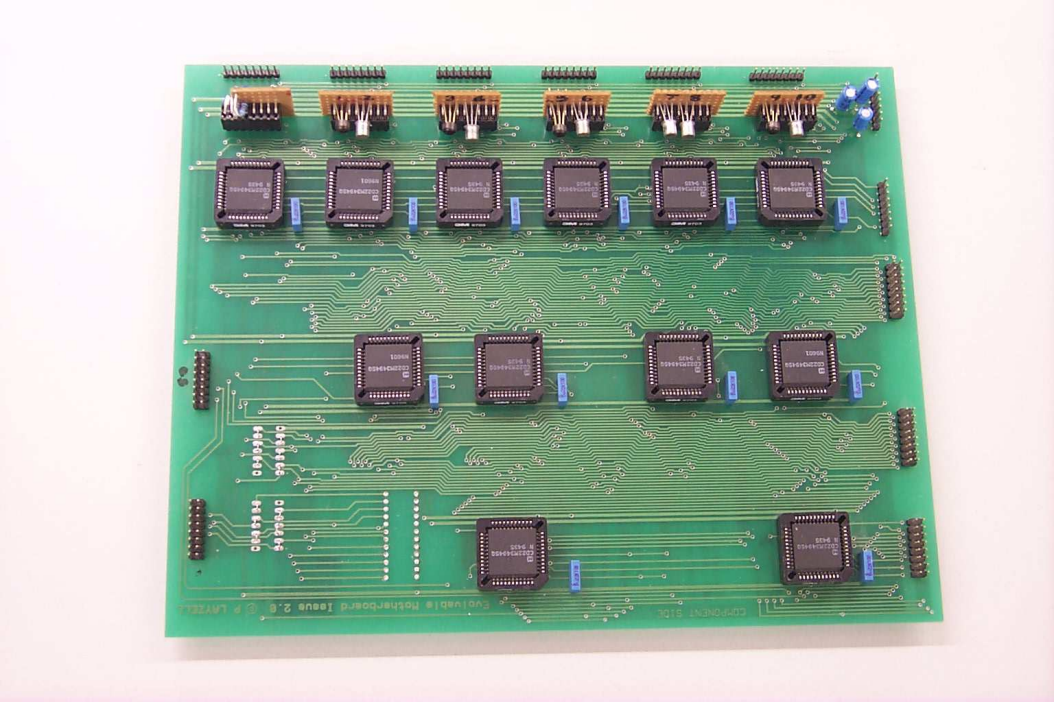
\includegraphics[height=10em]{tex/introduction/emradio.png}
\caption{
The physical programmable circuit used by Bird and Layzell \cite{Bird:2002:ERI:1251972.1252349} for solving the task of automatically designing oscillators.
}
\label{figs:emradio}
\end{figure}
% https://people.duke.edu/~ng46/topics/evolved-radio.pdf

\par \noindent (3)
\todo{toaster example}
% \cite{2017arXiv171209665B}
% https://arxiv.org/pdf/1712.09665.pdf
% https://arxiv.org/abs/1712.09665

\begin{figure}
\centering
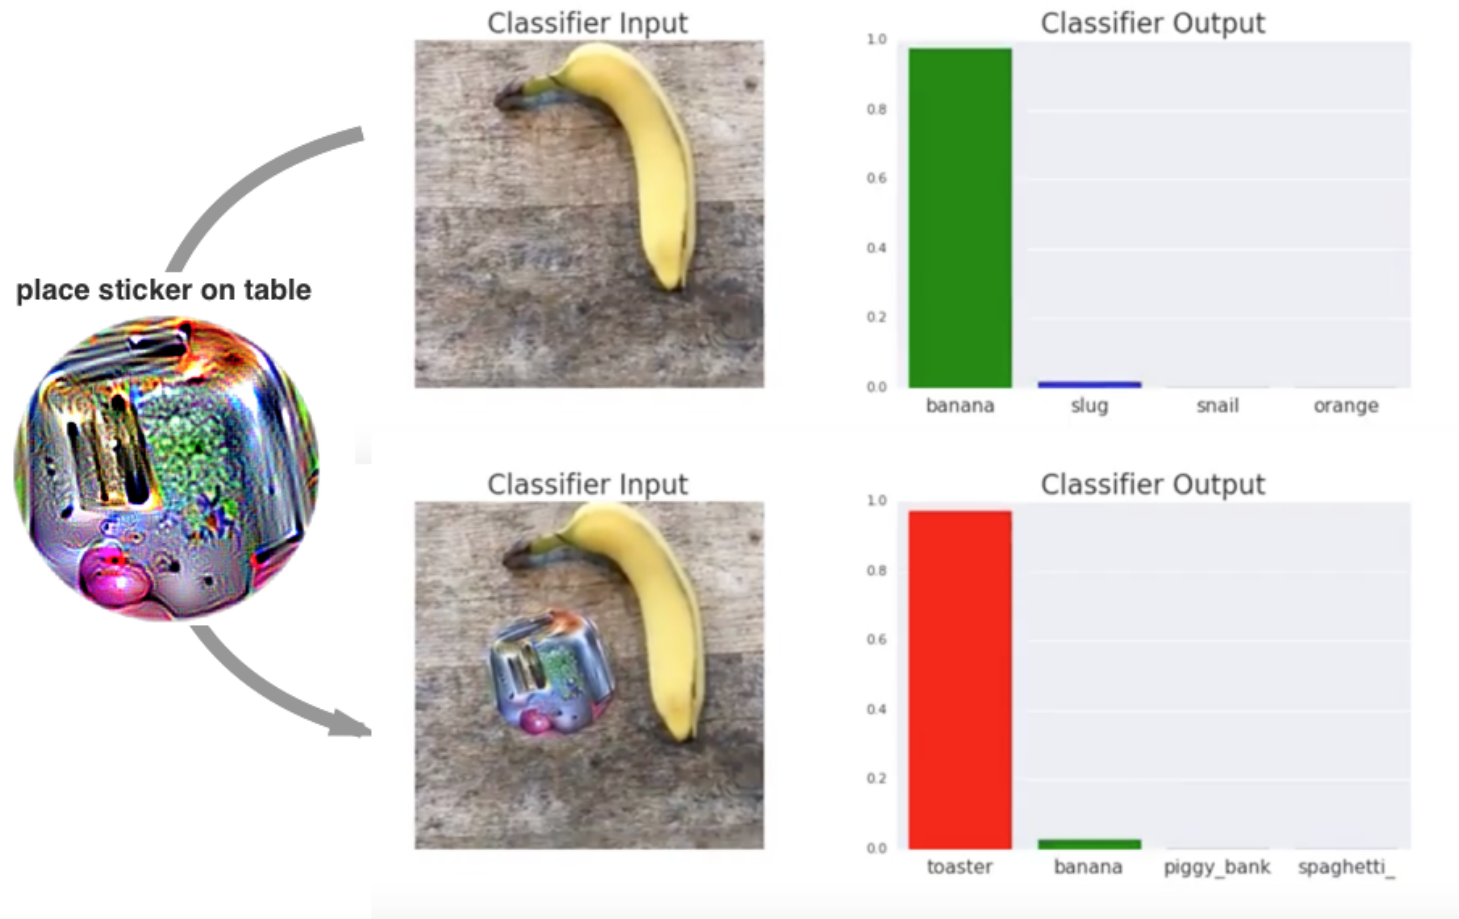
\includegraphics[height=10em]{tex/introduction/adversarialtoaster.png}
\caption{
\todo{TODO}
}
\label{figs:toaster}
\end{figure}

Those three examples all exhibit limitations of machine learning models where increasing the statistical accuracy of the model does not result in a semantically more correct model.
This is due to inherent biases of the data.

In the pneumonia example (1) patients with exceptionally high mortality risk were removed from the data leading to the model being unable to detect the severity of those cases.
In the radio example (2) the model utilized contextual data from the environment that is present but \emph{should} not be used in the model.
And in the toaster example (3) the model expected that all input data is coming from physical, real, objects.
Those biases cannot be detected from within the model or the data itself.
Furthermore, the process of detecting those errors, or even optimizing for semantic accuracy cannot be automated or be formulated as procedure, since there is no objective or measurable optimization criteria for it.
This is in contrast to statistical accuracy where a higher number always indicates a better model.
As a result, human judgment and contextual knowledge is absolutely necessary.

% There has been research...specialized models
% In order for a technique to be effectively useful for a human it needs to have few restrictions \todo{}
* black-box vs. white-box
* reasons for black box
\todo{problem statement}

The above example illustrates the need for human understanding and supervision in machine learning and the incorrect correct result could easily be identified since the authors used a special, intelligible, model. However, not all models used in machine learning are, or even attempt to be, easily interpretable by human experts. To counteract this, visual analytics has been successfully used to visualize machine learning processes in order to understand and gain insights into predictive models. Visual analytics is the area of studying interactive graphical representations of abstract information with the help of computational and statistical procedures, in order to effectively analyze complex data. With regards to understanding the decision making of predictive machine learning models, there are two main strategies: white-box and black-box analysis \cite{class_signatures}.

% \section{White-box vs. Black-box Analysis}
In white-box analysis the main focus lies in communicating the internal structure of the model at hand. That is, the analysis is based on the assumption that knowing the full internal state of a model and being able to manually retrace decisions made by it, helps understanding the \emph{behavior} of the model in general.

In this work we will focus on black-box analysis whose focus is on communicating external behavior of a model. That is, no information about the model itself is utilized during the analysis but rather typically inferred from observing how the model reacts to carefully crafted inputs. Compared to white-box analysis there are several advantages.

As white-box analysis relies on the internal structure and thus the nature of a particular model type, such as the $GA^2M$ mentioned above, a method developed for one type might not be applicable to a different type. This limits the usefulness of white-box analysis as every new algorithm demands often an entirely new form of representation. Since black-box analysis is model independent findings are universally applicable.

\newcommand\Tstrut{\rule{0pt}{2.5ex}}
\begin{table}
     \begin{tabular}{cl|cl} 
     & \textbf{White-box} & & \textbf{Black-box} \\
     \hline
     \hline
    $\oplus$ & Deep understanding of decisions & $\ominus$ & External behavior only \Tstrut \\
    $\oplus$ & Always reflects the true & $\ominus$ & Not guaranteed to reflect model \Tstrut \\
    & decision making process & & decisions truthfully in all cases \\
    $\oplus$ & Full internal state available & $\ominus$ & Limited knowledge of \Tstrut \\
    & & & model specifics \\
    \hline
    $\ominus$ & Model specific techniques & $\oplus$ & Reusable techniques \Tstrut \\
    $\ominus$ & Complexity / interpretability & $\oplus$ & Complexity / interpretability \Tstrut \\ 
    & data and model dependent & & independent of data and model \\
    $\ominus$ & Switching to interpretable model & $\oplus$ & No performance considerations \Tstrut \\
    & incurs performance penalty & & necessary \\
    \end{tabular}
    \centering
    \vspace*{-0.5em}
    \caption[Comparison of black-box and white-box explanation strategies.]{Comparison of black-box and white-box explanation strategies. $\oplus$ indicates advantages of a technique while $\ominus$ indicates drawbacks.}
    \vspace*{-0.75em}
    \label{tab:blackvswhite}
\end{table}

Another drawback of white-box analysis is its scalability to the complexity of the model. Many solutions do not sufficiently scale as models become more complex. For example, a decision tree with 5 nodes, often used as example when explaining the technique, can easily be visualized and understood in a node-link representation. This representation fails to help understanding a decision tree with hundreds or thousands of nodes. For black-box analysis the internal complexity of a model is irrelevant.

On the other hand black-box analysis also has drawbacks. Especially the limited knowledge of the underlying model allows only for an approximate understanding of its behavior as testing the entire input space would be intractable.